\documentclass[11pt,a4paper]{article}

\usepackage[margin=2.2cm]{geometry}
\usepackage{amsmath,amssymb,amsthm}
\usepackage{booktabs}
\usepackage{array}
\usepackage{tabularx}
\usepackage[shortlabels]{enumitem}
\usepackage{xcolor}
\usepackage{tikz}
\usepackage{fancyhdr}
\usepackage{setspace}
\usepackage{microtype}
\usepackage{titlesec}
\usepackage{hyperref}
\usepackage{listings}
\usepackage[skins,breakable]{tcolorbox}

\usetikzlibrary{positioning,arrows.meta,calc,fit,shapes.geometric,matrix,decorations.pathreplacing}

\definecolor{ink}{HTML}{222222}
\definecolor{rulegray}{HTML}{444444}
\definecolor{boxline}{HTML}{666666}
\definecolor{boxfill}{HTML}{F4F4F4}
\definecolor{boxtitle}{HTML}{E8E8E8}
\definecolor{g1}{HTML}{D0D0D0}
\definecolor{g2}{HTML}{9A9A9A}
\definecolor{g3}{HTML}{5A5A5A}

\hypersetup{
  colorlinks=true,
  linkcolor=black,
  urlcolor=black,
  pdftitle={MTL 458 Lecture 22: Persistence: Hard Disk Drives},
  pdfauthor={Minati De, IIT Delhi}
}

\setstretch{1.12}
\raggedbottom
\setlist[itemize]{leftmargin=1.3em,itemsep=0.28em,topsep=0.35em}
\setlist[enumerate]{leftmargin=1.5em,itemsep=0.35em,topsep=0.4em}

\titleformat{\section}
  {\Large\bfseries\color{ink}}{\thesection.}{0.6em}{}
  [{\color{rulegray}\titlerule[0.5pt]}]
\titleformat{\subsection}
  {\large\bfseries\color{ink}}{\thesubsection}{0.55em}{}
\titleformat{\subsubsection}
  {\normalsize\bfseries\color{ink}}{\thesubsubsection}{0.5em}{}

\titlespacing*{\section}{0pt}{1.35em}{0.7em}
\titlespacing*{\subsection}{0pt}{1.05em}{0.45em}

\pagestyle{fancy}
\fancyhf{}
\renewcommand{\headrulewidth}{0.4pt}
\renewcommand{\footrulewidth}{0.3pt}
\fancyhead[L]{\small\color{ink}MTL 458 \textbullet\ Operating Systems}
\fancyhead[R]{\small\color{ink}Lecture 22: Persistence: Hard Disk Drives}
\fancyfoot[C]{\small\thepage}
\setlength{\headheight}{14pt}

% ---------------------------------------------------------------------------
% Boxes
% ---------------------------------------------------------------------------
\tcbset{
  commonbox/.style={
    colback=boxfill, colframe=boxline, boxrule=0.5pt,
    left=6pt, right=6pt, top=5pt, bottom=5pt,
    fonttitle=\bfseries, coltitle=black, colbacktitle=boxtitle,
    enhanced, sharp corners=south, breakable
  }
}
\newtcolorbox{keybox}[1][]{commonbox, title={#1}}
\newtcolorbox{quizbox}[1][]{commonbox, title={#1}}
\newtcolorbox{solbox}[1][]{commonbox, title={#1}}
\newtcolorbox{warnbox}[1][]{commonbox, title={#1}}
\newtcolorbox{defbox}[1][]{commonbox, title={#1}}

% Start a new page unless at least #1 of vertical space remains
\makeatletter
\newcommand{\keepspace}[1]{\par\penalty-100\begingroup
  \setlength{\dimen@}{#1}\dimen@ii\pagegoal\advance\dimen@ii-\pagetotal
  \ifdim\dimen@>\dimen@ii\ifdim\dimen@ii>\z@\vfil\fi\break\fi\endgroup}
\makeatother

% ---------------------------------------------------------------------------
% Numbered platter (top view): 3 tracks x 8 sectors.
% \trackdisk{inner labels}{middle labels}{outer labels}{extra tikz}
% each label list has 8 entries, clockwise from 12 o'clock.
% Label positions are available as nodes i<k>, m<k>, o<k> (k = 0..7).
% ---------------------------------------------------------------------------
\newcommand{\trackdisk}[4]{%
\begin{tikzpicture}[scale=0.8]
  \fill[g2] (0,0) circle (2.05);
  \foreach \r in {0.95,1.5,2.05} \draw[white, line width=0.8pt] (0,0) circle (\r);
  \foreach \k in {0,...,7} \draw[white, line width=0.6pt] ({90-45*\k}:0.3) -- ({90-45*\k}:2.05);
  \foreach \lab [count=\k from 0] in {#1} \node[font=\scriptsize\bfseries, text=white] (i\k) at ({67.5-45*\k}:0.66) {\lab};
  \foreach \lab [count=\k from 0] in {#2} \node[font=\scriptsize\bfseries, text=white] (m\k) at ({67.5-45*\k}:1.23) {\lab};
  \foreach \lab [count=\k from 0] in {#3} \node[font=\scriptsize\bfseries, text=white] (o\k) at ({67.5-45*\k}:1.78) {\lab};
  \fill[black] (0,0) circle (0.3);
  #4
\end{tikzpicture}}
% head on the arm at angle #1, radius #2 (call inside the extra-tikz argument)
\newcommand{\diskhead}[2]{%
  \draw[line width=2.2pt, black!80] ($(#1:#2)!0.22cm!(215:2.9)$) -- (215:2.9);
  \fill[black!80] (215:2.9) circle (0.22);
  \draw[line width=1pt, black] (#1:#2) circle (0.22);}

\begin{document}

% ===========================================================================
% Title
% ===========================================================================
\begin{center}
{\small\itshape Made by Arpit's Milo}\\[0.3em]
{\color{rulegray}\rule{\textwidth}{1.1pt}}\\[0.45em]
{\LARGE\bfseries Operating Systems}\\[0.25em]
{\Large\bfseries MTL 458 \textperiodcentered\ Lecture 22}\\[0.35em]
{\LARGE\bfseries Persistence: Hard Disk Drives}\\[0.35em]
{\large Minati De}\\[0.15em]
{\normalsize Department of Mathematics, Indian Institute of Technology Delhi}\\[0.35em]
{\color{rulegray}\rule{\textwidth}{1.1pt}}
\end{center}

\vspace{0.4em}
\begin{keybox}[Questions]
\textbf{Answered in the last lecture:}
\begin{itemize}
  \item What are the components of a hard disk drive?
\end{itemize}
\textbf{Answered in this lecture:}
\begin{itemize}
  \item How can you calculate \textbf{sequential} and \textbf{random
        throughput} of a disk?
  \item What algorithms are used to \textbf{schedule I/O requests}?
\end{itemize}
\end{keybox}

\begingroup\small\setstretch{1.0}\tableofcontents\endgroup
\vspace{0.6em}
\noindent{\color{rulegray}\rule{\textwidth}{0.4pt}}

% ===========================================================================
\section{Review: the disk and the time to read/write}
% ===========================================================================

This section repeats the end of the previous lecture, which this lecture
builds on.

\subsection{Basic interface}

\begin{itemize}
  \item The disk has a \textbf{sector-addressable address space}: it appears
        as an \textbf{array of sectors}.
  \item Sectors are typically \textbf{512 bytes} or 4096 bytes.
  \item Main operations: \textbf{reads + writes to sectors}.
  \item The mechanical (slow) nature makes management ``interesting''.
\end{itemize}

\begin{center}
\trackdisk{0,1,2,3,4,5,6,7}{8,9,10,11,12,13,14,15}{16,17,18,19,20,21,22,23}{%
  \diskhead{180}{1.78}
  \draw[-{Latex}, thick] (60:2.35) arc[start angle=60, end angle=120, radius=2.35];
  \node[font=\small] at (90:2.65) {spin};}
\end{center}

\begin{itemize}
  \item \textbf{Heads} on a moving arm can read from each surface.
  \item The spindle/platters rapidly \textbf{spin} (counter-clockwise here,
        so the sectors of a track pass under the head in increasing order).
\end{itemize}

\subsection{Time to read/write}

\begin{keybox}[Three components]
\[
  \text{Time} \;=\; \text{seek} \;+\; \text{rotation} \;+\; \text{transfer time}
\]
\end{keybox}

\noindent\textbf{Seek}
\begin{itemize}
  \item Seek cost is a function of \textbf{cylinder distance}, but \textbf{not
        purely linear}: the arm must accelerate, coast, decelerate, settle.
  \item Settling alone can take \textbf{0.5--2 ms}; entire seeks often take
        several milliseconds, \textbf{4--10 ms}.
  \item Approximate average seek distance \(=\) \textbf{1/3 max seek
        distance}. (Why? If the start and target tracks are uniformly random
        on \([0,N]\), the expected distance \(|x-y|\) is \(N/3\); see the
        previous lecture for the integral.)
\end{itemize}

\noindent\textbf{Rotate}
\begin{itemize}
  \item Depends on rotations per minute (\textbf{RPM}); 7200 RPM is common,
        15000 RPM is high end.
  \item With 7200 RPM, how long to rotate around?
        \(1/7200\ \text{RPM} = 1\ \text{minute}/7200\ \text{rotations}
        = 1\ \text{second}/120\ \text{rotations} = 8.3\ \text{ms/rotation}\).
  \item Average rotation: \(8.3\ \text{ms}/2 = 4.15\ \text{ms}\) (on average
        the sector is half a turn away).
\end{itemize}

\noindent\textbf{Transfer}
\begin{itemize}
  \item Pretty fast: it depends on RPM and sector density. \textbf{100+
        MB/s} is typical for the maximum transfer rate.
  \item How long to transfer 512 bytes?
        \(512\ \text{bytes} \times (1\ \text{s}/100\ \text{MB}) \approx 5\
        \mu\text{s}\).
\end{itemize}

\subsection{Workload performance}

So\ldots\ \textbf{seeks are slow}, \textbf{rotations are slow},
\textbf{transfers are fast}. What kind of workload is fastest for disks?
\begin{itemize}
  \item \textbf{Sequential:} access sectors in order (\textbf{transfer
        dominated}).
  \item \textbf{Random:} access sectors arbitrarily (\textbf{seek + rotation
        dominated}).
\end{itemize}

% ===========================================================================
\section{Basic performance concepts}
% ===========================================================================

\begin{defbox}[Latency, throughput, overhead]
\begin{itemize}
  \item \textbf{Response time} or \textbf{latency}: time to perform an
        operation (s).
  \item \textbf{Bandwidth} or \textbf{throughput}: rate at which operations
        are performed (op/s). Files: MB/s; networks: Mb/s.
  \item \textbf{Start up} or ``\textbf{overhead}'': time to initiate an
        operation.
\end{itemize}
Most I/O operations are roughly linear:
\[
  \text{Latency}(n) \;=\; \text{Ovhd} \;+\; \frac{n}{\text{Bandwidth}}.
\]
\end{defbox}

For a disk, the overhead is the positioning time (seek + rotation) and the
\(n/\text{Bandwidth}\) term is the transfer time for \(n\) bytes. A large
\(n\) spreads the fixed overhead over many bytes; a small \(n\) makes the
overhead dominate. The next section shows this with numbers.

% ===========================================================================
\section{Disk throughput: worked examples}
% ===========================================================================

\subsection{Disk spec}

\begin{center}
\renewcommand{\arraystretch}{1.2}
\begin{tabular}{@{}lcc@{}}
  \toprule
   & \textbf{Cheetah} & \textbf{Barracuda} \\
  \midrule
  Capacity     & 300 GB   & 1 TB \\
  RPM          & 15,000   & 7,200 \\
  Avg Seek     & 4 ms     & 9 ms \\
  Max Transfer & 125 MB/s & 105 MB/s \\
  Platters     & 4        & 4 \\
  Cache        & 16 MB    & 32 MB \\
  \bottomrule
\end{tabular}
\end{center}

\keepspace{9\baselineskip}
\begin{quizbox}[Sequential workload: what is the throughput for each?]
In a sequential workload the disk positions once and then just streams
sectors, so throughput is the \textbf{maximum transfer rate}:
\begin{itemize}
  \item Cheetah: \textbf{125 MB/s};
  \item Barracuda: \textbf{105 MB/s}.
\end{itemize}
\end{quizbox}

\begin{quizbox}[Random workload: what is the throughput for each? (What else do you need to know?)]
We need the \textbf{size of each random read}, because every request pays
the full seek and rotation and then transfers only that much data.
\textbf{Assume 16-KB reads.}
\end{quizbox}

\keepspace{18\baselineskip}
\subsection{Cheetah: an average random 16-KB read}

\begin{solbox}[How long does an average random 16-KB read take with Cheetah?]
Time \(=\) seek \(+\) rotation \(+\) transfer.
\begin{itemize}
  \item \textbf{Seek} \(= 4\) ms (average seek from the spec).
  \item \textbf{Average rotation} (half a rotation at 15,000 RPM):
  \[
    \frac12 \times \frac{1\ \text{min}}{15000} \times \frac{60\ \text{sec}}{1\ \text{min}}
    \times \frac{1000\ \text{ms}}{1\ \text{sec}} = 2\ \text{ms}.
  \]
  \item \textbf{Transfer of 16 KB:}
  \[
    \frac{1\ \text{sec}}{125\ \text{MB}} \times 16\ \text{KB} \times
    \frac{1\ \text{MB}}{1024\ \text{KB}} \times
    \frac{1{,}000{,}000\ \mu\text{s}}{1\ \text{sec}} = 125\ \mu\text{s}.
  \]
  \item \textbf{Total:} Cheetah time \(= 4\ \text{ms} + 2\ \text{ms} +
        125\ \mu\text{s} \approx 6.1\ \text{ms}\).
  \item \textbf{Throughput:}
  \[
    \frac{16\ \text{KB}}{6.1\ \text{ms}} \times \frac{1\ \text{MB}}{1024\ \text{KB}}
    \times \frac{1000\ \text{ms}}{1\ \text{sec}} \approx 2.5\ \text{MB/s}.
  \]
\end{itemize}
{\small (The slide writes ``100 ms / 1 sec'' in the last factor; it must be
1000 ms / 1 sec to get 2.5 MB/s.)}
\end{solbox}

\keepspace{18\baselineskip}
\subsection{Barracuda: an average random 16-KB read}

\begin{solbox}[How long does an average random 16-KB read take with Barracuda?]
Time \(=\) seek \(+\) rotation \(+\) transfer.
\begin{itemize}
  \item \textbf{Seek} \(= 9\) ms.
  \item \textbf{Average rotation} (half a rotation at 7,200 RPM):
  \[
    \frac12 \times \frac{1\ \text{min}}{7200} \times \frac{60\ \text{sec}}{1\ \text{min}}
    \times \frac{1000\ \text{ms}}{1\ \text{sec}} \approx 4.1\ \text{ms}.
  \]
  \item \textbf{Transfer of 16 KB:}
  \[
    \frac{1\ \text{sec}}{105\ \text{MB}} \times 16\ \text{KB} \times
    \frac{1\ \text{MB}}{1024\ \text{KB}} \times
    \frac{1{,}000{,}000\ \mu\text{s}}{1\ \text{sec}} \approx 149\ \mu\text{s}.
  \]
  \item \textbf{Total:} Barracuda time \(= 9\ \text{ms} + 4.1\ \text{ms} +
        149\ \mu\text{s} \approx 13.2\ \text{ms}\).
  \item \textbf{Throughput:}
  \[
    \frac{16\ \text{KB}}{13.2\ \text{ms}} \times \frac{1\ \text{MB}}{1024\ \text{KB}}
    \times \frac{1000\ \text{ms}}{1\ \text{sec}} \approx 1.2\ \text{MB/s}.
  \]
\end{itemize}
\end{solbox}

\subsection{Sequential vs.\ random}

\begin{center}
\renewcommand{\arraystretch}{1.2}
\begin{tabular}{@{}lcc@{}}
  \toprule
   & \textbf{Cheetah} & \textbf{Barracuda} \\
  \midrule
  Sequential & 125 MB/s & 105 MB/s \\
  Random     & 2.5 MB/s & 1.2 MB/s \\
  \bottomrule
\end{tabular}
\end{center}

\begin{keybox}[Takeaway]
Random throughput is about \textbf{50--90 times lower} than sequential
throughput on the same disk: with 16-KB random reads, almost all the time
goes to seek and rotation (6 ms out of 6.1 ms on the Cheetah), not to
transferring data.
\end{keybox}

% ===========================================================================
\section{Other improvements}
% ===========================================================================

Three hardware techniques make disks faster: \textbf{track skew},
\textbf{zones}, and a \textbf{cache}.

\keepspace{30\baselineskip}
\subsection{Track skew}

\begin{quizbox}[Imagine sequential reading: how should sector numbers be laid out on disk?]
Suppose we read sectors 0, 1, 2, \ldots\ in order. Sector 15 is the last
sector of the middle track, and sector 16 is the first sector of the outer
track. To go from 15 to 16 the head must move to the next track (a short
seek) and \textbf{settle} there.
\end{quizbox}

\begin{center}
\begin{minipage}[t]{0.47\textwidth}\centering
\trackdisk{,,,,,,,}{8,9,10,11,12,13,14,\textbf{15}}{\textbf{16},17,18,19,20,21,22,23}{%
  \diskhead{180}{1.78}
  \draw[-{Latex}, very thick] (m7.north) to[bend left=40] (o0.north);}\\[0.2em]
{\small (a) No skew: 16 is right next to 15. When reading 16 after 15,
the head won't settle quick enough, so we need to do a rotation.}
\end{minipage}\hfill
\begin{minipage}[t]{0.47\textwidth}\centering
\trackdisk{,,,,,,,}{8,9,10,11,12,13,14,\textbf{15}}{22,23,\textbf{16},17,18,19,20,21}{%
  \diskhead{180}{1.78}
  \draw[-{Latex}, very thick] (m7.north) .. controls (85:3.3) and (5:3.2) .. (o2.east);}\\[0.2em]
{\small (b) Track skew: the outer track is rotated by two sectors, so 16
arrives later: enough time to settle now.}
\end{minipage}
\end{center}

\begin{itemize}
  \item \textbf{Without skew} (a): after 15 has passed under the head, 16 is
        the very next sector to arrive. The head is still moving and settling
        on the outer track, so 16 has already gone by. The disk must wait
        almost a \textbf{full extra rotation} for 16 to come back.
  \item \textbf{With track skew} (b): the start of each track is offset by a
        few sectors. While the head switches tracks and settles, sectors 22
        and 23 pass under it; then 16 arrives just in time.
\end{itemize}
{\small (Sectors are numbered clockwise and the disk spins
counter-clockwise, so the head meets the numbers in increasing order. The
inner track is left unnumbered in these frames, as on the slides. The slide
for (b) prints ``23'' twice in the outer ring; the left one should be 22, as
drawn here.)}

\keepspace{22\baselineskip}
\subsection{Zones}

\begin{center}
\begin{minipage}[t]{0.23\textwidth}\centering

\begin{tikzpicture}[scale=0.48]
  \fill[g2] (0,0) circle (2.05);
  \foreach \r in {0.5,1.0,1.5,2.05} \draw[white, line width=0.8pt] (0,0) circle (\r);
\end{tikzpicture}\\
{\small (a) A platter is rings of tracks.}
\end{minipage}\hfill
\begin{minipage}[t]{0.23\textwidth}\centering
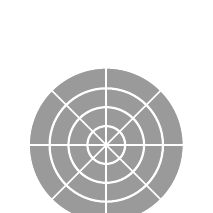
\begin{tikzpicture}[scale=0.48]
  \fill[g2] (0,0) circle (2.05);
  \foreach \r in {0.5,1.0,1.5,2.05} \draw[white, line width=0.8pt] (0,0) circle (\r);
  \foreach \k in {0,...,7} \draw[white, line width=0.6pt] (0,0) -- ({45*\k}:2.05);
\end{tikzpicture}\\
{\small (b) Divided into equal sectors: 8 on every track.}
\end{minipage}\hfill
\begin{minipage}[t]{0.23\textwidth}\centering
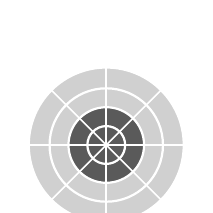
\begin{tikzpicture}[scale=0.48]
  \fill[g1] (0,0) circle (2.05);
  \fill[g3] (0,0) circle (1.0);
  \foreach \r in {0.5,1.0,1.5,2.05} \draw[white, line width=0.8pt] (0,0) circle (\r);
  \foreach \k in {0,...,7} \draw[white, line width=0.6pt] (0,0) -- ({45*\k}:2.05);
\end{tikzpicture}\\
{\small (c) Two zones, still 8 sectors per track.}
\end{minipage}\hfill
\begin{minipage}[t]{0.23\textwidth}\centering
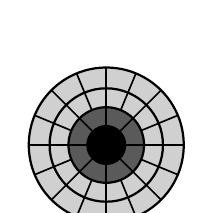
\begin{tikzpicture}[scale=0.48]
  \fill[g1] (0,0) circle (2.05);
  \fill[g3] (0,0) circle (1.0);
  \foreach \r in {0.5,1.0,1.5,2.05} \draw[black, line width=0.8pt] (0,0) circle (\r);
  \foreach \k in {0,...,7} \draw[black, line width=0.6pt] (0,0) -- ({45*\k}:2.05);
  \foreach \k in {0,...,7} \draw[black, line width=0.6pt] ({45*\k+22.5}:1.0) -- ({45*\k+22.5}:2.05);
  \fill[black] (0,0) circle (0.5);
\end{tikzpicture}\\
{\small (d) \textbf{ZBR}: 16 sectors outer, 8 inner.}
\end{minipage}
\end{center}

\begin{defbox}[ZBR (zoned bit recording)]
\textbf{More sectors on outer tracks.} An outer track is longer than an
inner track. If every track had the same number of sectors, the outer
tracks would store bits much less densely than the inner ones and waste
space. So tracks are grouped into \textbf{zones}: all tracks in a zone have
the same number of sectors, and zones further out have more sectors per
track.
\end{defbox}

\subsection{Drive cache}

\noindent
\begin{minipage}{0.6\textwidth}
\begin{itemize}
  \item Drives may cache both reads and writes.
  \item The OS caches data too.
\end{itemize}
\end{minipage}\hfill
\begin{minipage}{0.35\textwidth}\centering
\scalebox{0.7}{\trackdisk{,,,,,,,}{8,9,10,11,12,13,14,15}{16,17,18,19,20,21,22,23}{}}\\[0.2em]
{\small (one track can be read into the drive's track buffer)}
\end{minipage}

\keepspace{13\baselineskip}
\begin{quizbox}[What advantage does caching in the \emph{drive} have for reads? For writes?]
\begin{itemize}
  \item \textbf{Reads:} the drive can \textbf{read ahead}. While it waits for
        the requested sector to rotate under the head, it reads the rest of
        the track into its cache. Later sequential reads are then served from
        the cache with no seek or rotation.
  \item \textbf{Writes:} the drive can report a write as done as soon as the
        data is in its cache, and write it to the platter later. The writer
        gets a fast response, but the data can be lost if power fails before
        it reaches the platter.
\end{itemize}
\end{quizbox}

\subsection{Buffering}

\begin{itemize}
  \item Disks contain internal memory (2 MB--16 MB) used as a cache.
  \item \textbf{Read-ahead: ``track buffer''.}
    \begin{itemize}
      \item Read the contents of the entire track into memory during the
            rotational delay.
    \end{itemize}
  \item \textbf{Write caching with volatile memory.}
    \begin{itemize}
      \item \textbf{Immediate reporting:} claim the data is written to disk
            when it is not;
      \item data could be lost on power failure.
    \end{itemize}
  \item \textbf{Tagged command queueing.}
    \begin{itemize}
      \item Have multiple outstanding requests to the disk;
      \item the disk can reorder (schedule) requests for better performance.
    \end{itemize}
\end{itemize}

% ===========================================================================
\section{I/O schedulers}
% ===========================================================================

\begin{keybox}[The scheduling problem]
Given a stream of I/O requests, in what order should they be served?
\begin{itemize}
  \item This is much different from CPU scheduling.
  \item The \textbf{position of the disk head relative to the request
        position} matters more than the length of the job.
\end{itemize}
\end{keybox}

\subsection{FCFS (First-Come-First-Serve)}

\begin{quizbox}[How long (roughly) does the workload below take?]
Assume seek + rotate \(= 10\) ms for a random request. Requests are given in
sector numbers.

\medskip
\renewcommand{\arraystretch}{1.25}
\begin{tabular}{@{}ll@{}}
  \textbf{FCFS order:} & 300001, 700001, 300002, 700002, 300003, 700003
      \quad\(\Rightarrow\)\quad \textbf{\(\sim\)60 ms} \\
  \textbf{Reordered:} & 300001, 300002, 300003, 700001, 700002, 700003
      \quad\(\Rightarrow\)\quad \textbf{\(\sim\)20 ms} \\
\end{tabular}

\medskip
In FCFS order the head jumps between the two far-apart regions on
\emph{every} request: 6 random requests \(\times\) 10 ms \(\approx\) 60 ms.
Served in sorted order, there are only two random positionings (one to
300001, one to 700001); the rest are the next sectors, which cost almost
nothing: \(2 \times 10\) ms \(\approx\) 20 ms. \textbf{Order matters a
lot.}
\end{quizbox}

\subsection{Where should the scheduler go?}

\begin{center}
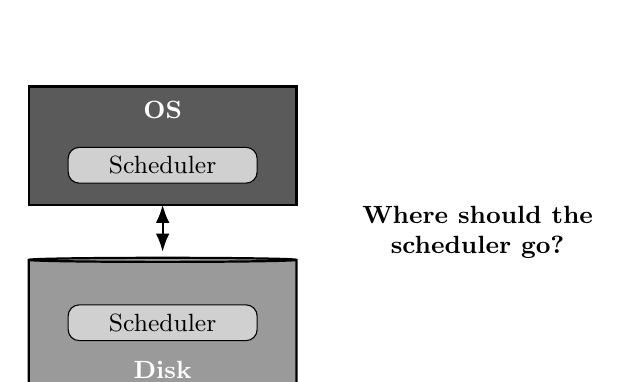
\begin{tikzpicture}
  \node[draw, thick, fill=g3, text=white, minimum width=3.4cm, minimum height=1.5cm,
        label={[font=\small\bfseries, text=white]above:{}}] (os) at (0,2.3) {};
  \node[font=\small\bfseries, text=white] at (0,2.75) {OS};
  \node[draw, rounded corners, fill=g1, font=\small, minimum width=2.4cm] at (0,2.05) {Scheduler};
  \node[cylinder, shape border rotate=90, aspect=0.22, draw, thick, fill=g2,
        minimum width=3.4cm, minimum height=1.7cm] (dk) at (0,0) {};
  \node[draw, rounded corners, fill=g1, font=\small, minimum width=2.4cm] at (0,0.05) {Scheduler};
  \node[font=\small\bfseries, text=white] at (0,-0.55) {Disk};
  \draw[{Latex}-{Latex}, thick] (0,1.55) -- (0,0.95);
  \node[font=\small\bfseries, align=center] at (4,1.2) {Where should the\\scheduler go?};
\end{tikzpicture}
\end{center}

Both places have a scheduler, and each knows something the other doesn't:
\begin{itemize}
  \item The \textbf{OS} knows about processes, priorities and fairness, but
        it does not know the disk's exact geometry or where the head is in
        its rotation.
  \item The \textbf{disk} knows its own geometry and the current head and
        rotational position exactly. With tagged command queueing it can
        reorder the requests it has been given.
\end{itemize}

\subsection{SPTF (Shortest Positioning Time First)}

\begin{itemize}
  \item \textbf{Strategy:} always choose the request that requires the least
        \textbf{positioning time} (time for seeking and rotating).
  \item \textbf{Greedy} algorithm: it just looks for the best NEXT decision.
  \item \textbf{How to implement in the disk?} The disk knows both seek and
        rotational costs, so it can run SPTF directly.
  \item \textbf{How to implement in the OS?} The OS does not know rotation
        times, so it uses \textbf{Shortest Seek Time First (SSTF)} instead:
        it picks the request on the nearest track (by cylinder distance).
  \item \textbf{Disadvantages?} It is easy for far-away requests to
        \textbf{starve}. While requests keep arriving near the head, a
        request on a distant track is never the closest one.
\end{itemize}

\subsection{SCAN}

\begin{itemize}
  \item \textbf{Elevator algorithm:} sweep back and forth, from one end of
        the disk to the other, serving requests as the head passes that
        cylinder.
  \item Sorts by cylinder number; \textbf{ignores rotation delays}.
\end{itemize}

\begin{quizbox}[Pros/cons?]
\textbf{Pro:} no starvation. Every request is served within one sweep in
each direction, because the head never turns back before reaching the end.

\textbf{Cons:} it ignores rotation, so it can be worse than SPTF. It is also
not fair to all tracks: the middle tracks are passed twice per round trip
(once in each direction), while tracks at the ends wait for a full trip.
\end{quizbox}

\textbf{Better: C-SCAN (circular scan).} Only sweep in one direction: serve
requests from one end to the other, then jump back to the start and sweep
again. Every track then waits about the same time.

\subsection{Work conservation}

\begin{itemize}
  \item \textbf{Work-conserving schedulers} always try to do work if there's
        work to be done.
  \item Sometimes it's better to \textbf{wait} instead, if the system
        \textbf{anticipates} another request will arrive (e.g.\ the next
        sequential read from the same process, which would be nearly free).
  \item Such \textbf{non-work-conserving} schedulers are called
        \textbf{anticipatory schedulers}.
\end{itemize}

\subsection{CFQ (Linux default)}

CFQ was the Linux default when these slides were written; newer kernels have
removed it in favour of multi-queue schedulers such as BFQ and mq-deadline.

\textbf{Completely Fair Queueing:}
\begin{itemize}
  \item a queue for each process;
  \item weighted round-robin between queues, with slice time proportional to
        priority;
  \item yield the slice only if idle for a given time (\textbf{anticipation});
  \item optimize the order within each queue.
\end{itemize}

\keepspace{20\baselineskip}
% ===========================================================================
\section{I/O device summary}
% ===========================================================================

\begin{keybox}[Summary]
\begin{itemize}
  \item \textbf{Overlap I/O and CPU whenever possible!} Use interrupts and
        DMA.
  \item Storage devices provide a \textbf{common block interface}.
  \item On a disk: \textbf{never do random I/O unless you must!} E.g.,
        Quicksort is a terrible algorithm on disk, because it jumps around
        the data.
  \item Spend time to \textbf{schedule} on slow, stateful devices.
\end{itemize}
\end{keybox}

\begin{center}
\renewcommand{\arraystretch}{1.2}
\small
\begin{tabularx}{\textwidth}{@{}lX@{}}
  \toprule
  \textbf{Topic} & \textbf{Key facts} \\
  \midrule
  Access time & seek + rotation + transfer; seek 4--10 ms, avg rotation = half a turn \\
  Sequential throughput & = max transfer rate (Cheetah 125 MB/s, Barracuda 105 MB/s) \\
  Random throughput & size / (seek + rotation + transfer); 16 KB: 2.5 MB/s and 1.2 MB/s \\
  Track skew & offset each track's sector 0 so the head can settle after a track switch \\
  Zones (ZBR) & more sectors on outer tracks \\
  Drive cache & read-ahead track buffer; write caching with immediate reporting (risky); tagged command queueing \\
  FCFS & serves in arrival order; can be very slow \\
  SPTF / SSTF & greedy nearest-first (in disk / in OS); can starve far requests \\
  SCAN / C-SCAN & elevator sweeps; C-SCAN sweeps one way only \\
  Anticipatory & non-work-conserving: wait briefly for a likely nearby request \\
  CFQ & per-process queues, weighted round-robin, anticipation \\
  \bottomrule
\end{tabularx}
\end{center}

\end{document}
